\glsresetall{} 
\appendix

\chapter{Algorithms}

Through the development of the \gls{pops}, a number of algorithms have been
developed to perform various functions. These algorithms are not necessarily
ground breaking but their implementations are novel and worth discussing in
some form. To avoid detracting from the main body of the thesis they have been
placed here, in the appendices.


\section{Algorithm 1: Multiple Access Intersection} 

For some search scenarios, we may need to determine for what times do all
satellites have access to an \gls{aoi} or a ground station. That is, if we have
more than one satellite and each satellite has a list of access times to an
AOI, we must generate a new list of access times where each access corresponds
to a period where all satellites have access. An  example scenario is
illustrated in Figure \ref{fig:access_intersect}.


\begin{figure}[h]
    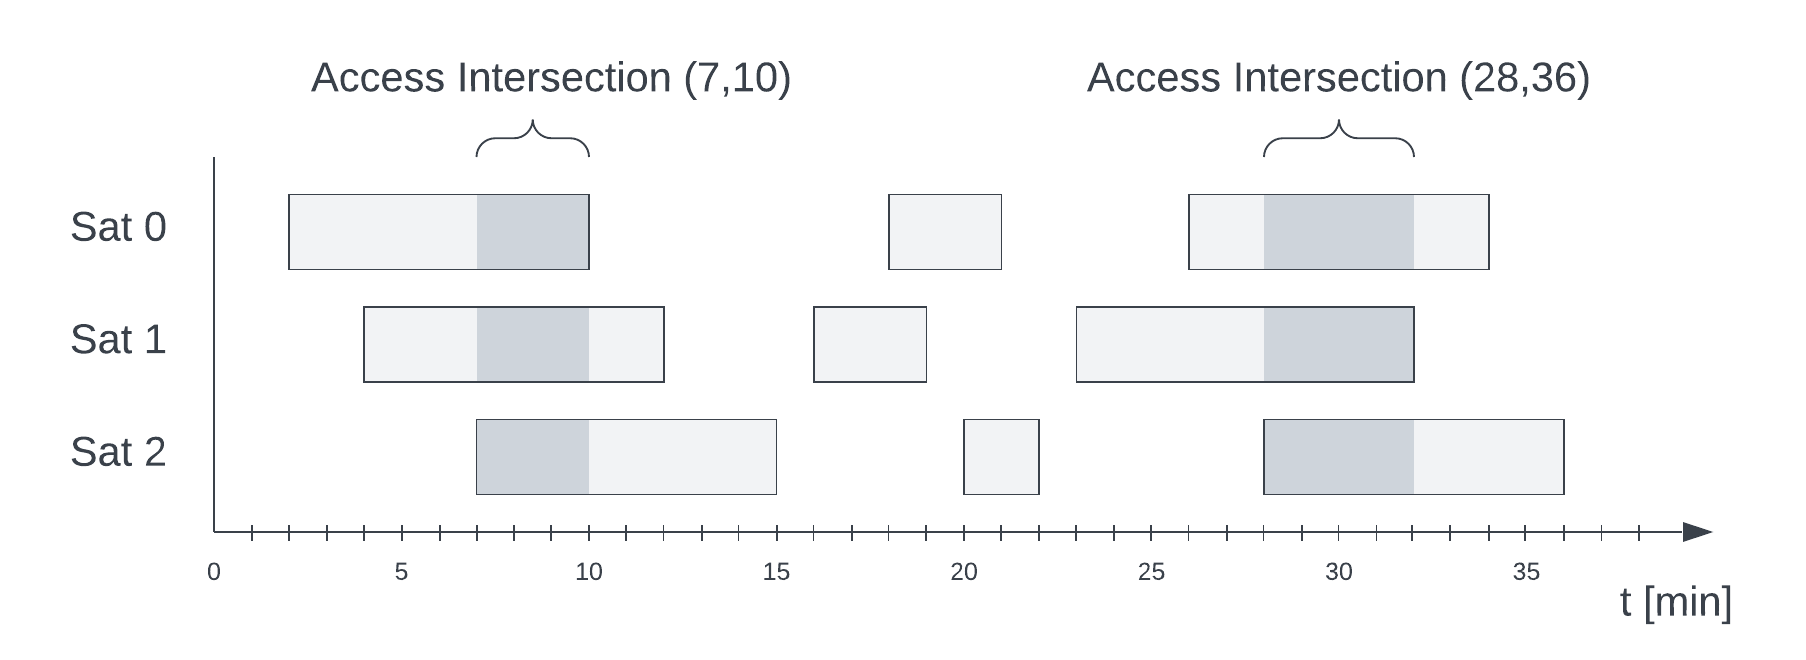
\includegraphics[width=\textwidth]{Access Intersection Example.png} 
    \caption{Illustration of a Potential Access Intersection Scenario}
\label{fig:access_intersect}
\end{figure}

In this scenario, there are three satellites: Sat 0, Sat 1, and Sat 2. Each has
multiple access periods represented with grey boxes. Though time is continuous,
it has been discretized into integer timesteps for simplicity. Minutes have
been selected as the units for time but this is arbitrary. From these lists of
access periods, this algorithm must determine all of the points in time where
all satellites have an access period. For the example scenario, the outputted
results should be $(7,10)$ and $(28,36)$. Note that between $t = $


For a satellite, access times are stored as a list of timestamps. Every even
and odd indexed timestamp specifies when the satellite `enters' and `leaves' an
access respectively. Access lists $A_n$ can be described generally for satellite $n$ as,

$$
A_n = \left[ \, a_{n,0}, \, b_{n,0}, \, a_{n,1}, \, b_{n,1}, \, \ldots \, a_{n,m}, \, b_{n,m} \, \right]
$$ 

where $a$ is the access enter timestamp, $b$ is the access leave timestamp,
and $m$ is the number of accesses.



